\documentclass[12pt,twoside]{article}
\usepackage[dvipsnames]{xcolor}
\usepackage{tikz,graphicx,amsmath,amsfonts,amscd,amssymb,bm,cite,epsfig,epsf,url}
\usepackage[hang,flushmargin]{footmisc}
\usepackage[colorlinks=true,urlcolor=blue,citecolor=blue]{hyperref}
\usepackage{amsthm,multirow,wasysym,appendix}
\usepackage{array,subcaption} 
% \usepackage[small,bf]{caption}
\usepackage{bbm}
\usepackage{pgfplots}
\usetikzlibrary{spy}
\usepgfplotslibrary{external}
\usepgfplotslibrary{fillbetween}
\usetikzlibrary{arrows,automata}
\usepackage{thmtools}
\usepackage{blkarray} 
\usepackage{textcomp}
\usepackage[left=0.8in,right=1.0in,top=1.0in,bottom=1.0in]{geometry}
\newcommand{\ry}{\rnd{ y}  }
\newcommand{\rx}{\rnd{ x}  }
\newcommand{\ru}{\rnd{ u}  }
\newcommand{\rd}{\rnd{ d}  }
%\newcommand{\rs}{\rnd{ s}  }
\newcommand{\ri}{\rnd{ i}  }
\newcommand{\re}{\rnd{ e}  }
\newcommand{\rQ}{\rnd{ q}  }
\newcommand{\rC}{\rnd{ c}  }
\newcommand{\rnd}{\Tilde}
\usepackage{pdfpages}
\title{1002 HW 9}
\author{gjd9961 }
\date{December 4th 2021}
\begin{document}
\maketitle
\begin{enumerate}

\item (Noisy measurement)
We are interested in measuring a certain quantity modeled by a random variable $\rx$ with zero mean and unit variance. Our available measurements $\ry: = \rx + \rnd{z}$ are corrupted by additive random noise, modeled as a random variable $\rnd{z}$ with zero mean and variance $\sigma^2$, which is independent from $\rx$.  
\begin{enumerate}
\item What is the best linear estimate of $\rx$ given $\ry = y$?
\subitem
So we can compute this using the general linear estimate formula and then capitalize on the fact that x is a standardized random variable and that since the mean of x and y is 0 then the variance is just the expectation of each respective variable squared. We can also take advantage of the fact that x and z are independent. 
\begin{equation}
    \begin{split}
        \arg \min_\alpha E((x-\alpha y)^2) &= E(x^2 + \alpha^2y^2 - 2\alpha yx)\\
        &= E(x^2) + \alpha^2E(y^2) - 2\alpha E(xy) \\
        &= E(x^2) + \alpha^2E(y^2) - 2\alpha E(x(x+z) \\
        &= E(x^2) + \alpha^2E(y^2) - 2\alpha E(x^2) - 2\alpha E(xz) \\
        &= E(x^2) + \alpha^2E(y^2) - 2\alpha E(x^2) - 2\alpha E(xz) \\
        &= 1 + \alpha^2E(y^2) - 2\alpha
    \end{split}
\end{equation}
Taking the derivative with respect to $\alpha$ and setting the equation to 0 we get that the best value for $\alpha$ is:
$$
    \alpha = \frac{1}{E(y^2)}
$$
So we now must compute the mean and variance of y.
$$
    E(y) = E(x+z) = E(x) + E(y) = 0 + 0 = 0
$$
$$
    Var(y) = E(y^2) + E^2(y) = E(y^2) = E((x+z)^2) = E(x^2) + E(z^2) + 2E(xy) = 1 + \sigma^2
$$
Therefore the best estimate for alpha is:
$$
    \alpha = \frac{1}{1 + \sigma^2}
$$
And our best linear estimate for $x$ given $y=y$ is:
$$
    x = \frac{1}{1 + \sigma^2}y
$$
\item What is the corresponding mean squared error?
The mean square error is given by the following equation, which we plug $alpha$ into:
$$
    MSE = (1-\rho_{x,y})\sigma_x^2 = 1 - \frac{1}{1+\sigma^2}
$$
\item What happens to the estimate and the error when $\sigma \rightarrow 0$? Explain why this makes sense. 
\subitem
As sigma approaches 0 we our mean square error will approach 0 as well, and we will have no prediction error. This is because we would effectively be eliminating the variance from our noise variable, and since it the noise variable z has mean of 0, thus this would indicate we are taking perfect measurements of x with y, so our prediction would be spot on. 
\item What happens to the estimate and the error when $\sigma \rightarrow \infty$? Explain why this makes sense. 
\subitem When sigma approaches infinity then the mean square error is 1 and the alpha term in our linear estimate becomes 0. Thus our estimate is 0, which happens to be the mean of x. This makes sense as since the variance of the noise variable z is so large, it makes y an unreliable predictor. It better suits us to guess the mean of x in this scenario.
\end{enumerate}


\item (Rufus)
\begin{figure}[h]
\begin{center}
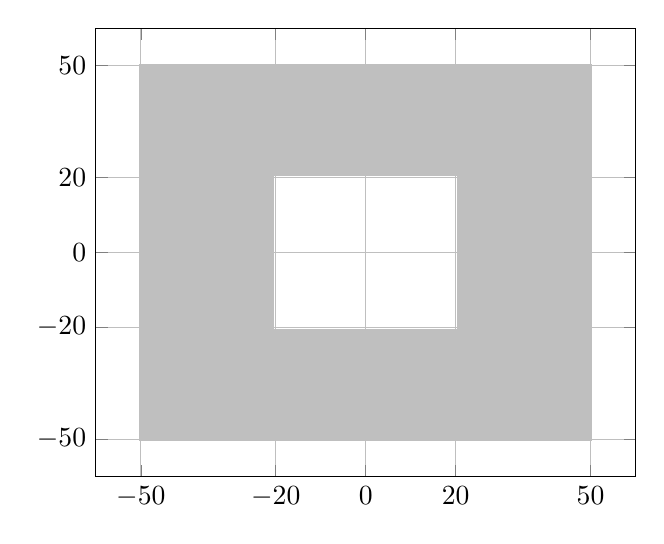
\begin{tikzpicture}
\begin{axis}[grid=major, xtick={-50,-20,0,20,50}, ytick={-50,-20,0,20,50}, xmin= -60, xmax=60, ymin=-60, ymax=60,axis on top]
\addplot[ fill, very thick, lightgray] coordinates
{(-50,50) (-50,-50) (50,-50) (50,50) } --cycle;
\addplot[fill, very thick, white] coordinates
{(-20,20) (-20,-20) (20,-20) (20,20) } --cycle;
\end{axis}
\end{tikzpicture}
\end{center}
\caption{Nora's garden (in gray).}
\label{fig:garden}
\end{figure}
Nora's dog Rufus lives in her garden, which is the shaded area in Figure~\ref{fig:garden}. After observing Rufus for a while she decides that his position within the garden is uniformly distributed (i.e. the probability density of his position is the same at every point of the garden). Let $\rx$ be the position of Rufus on the x axis in Figure~\ref{fig:garden} and $\ry$ his position on the y axis.
\begin{enumerate}
\item Compute the mean of $\rx$.
\subitem Short answer: the mean of $\rx$ is 0. We can clearly see this as the uniform distribution that models Rufus' position around the garden is centered about 0 and symmetric. We can compute this more rigorously in the following way once we calculate the pdf of $\rx$ and $\ry$.

\item Compute the pdf of $\ry$. Sketch it. 
\subitem We only need to consider two separate $\ry$ positions for Rufus, those that are bounded when x is between $[-50,-20]$ (which will work for the position bounded by $[20,50]$ as the distribution is unifrom and symmetric), and those that are bounded when x is between $[-20,20]$.\\
Firstly we calculate the pdf of $\ry$ for $[-50,-20]$ / $[20,50]$:
$$
    \int_{x=-50}^{x=50} f_{\rx,]\ry}(\rx,\ry)dx = \int_{x=-50}^{x=50} \frac{1}{8400} = \frac{100}{8400} = \frac{1}{84}
$$
Now we calculate the pdf of $\ry$ for $[-20,20]$:
$$
    \int_{x=-50}^{x=20} f_{\rx,]\ry}(\rx,\ry)dx = \int_{x=-50}^{x=20} \frac{1}{8400} = 2*\frac{30}{8400} = \frac{1}{140}
$$
Otherwise the pdf is 0. PDF of $\ry$:

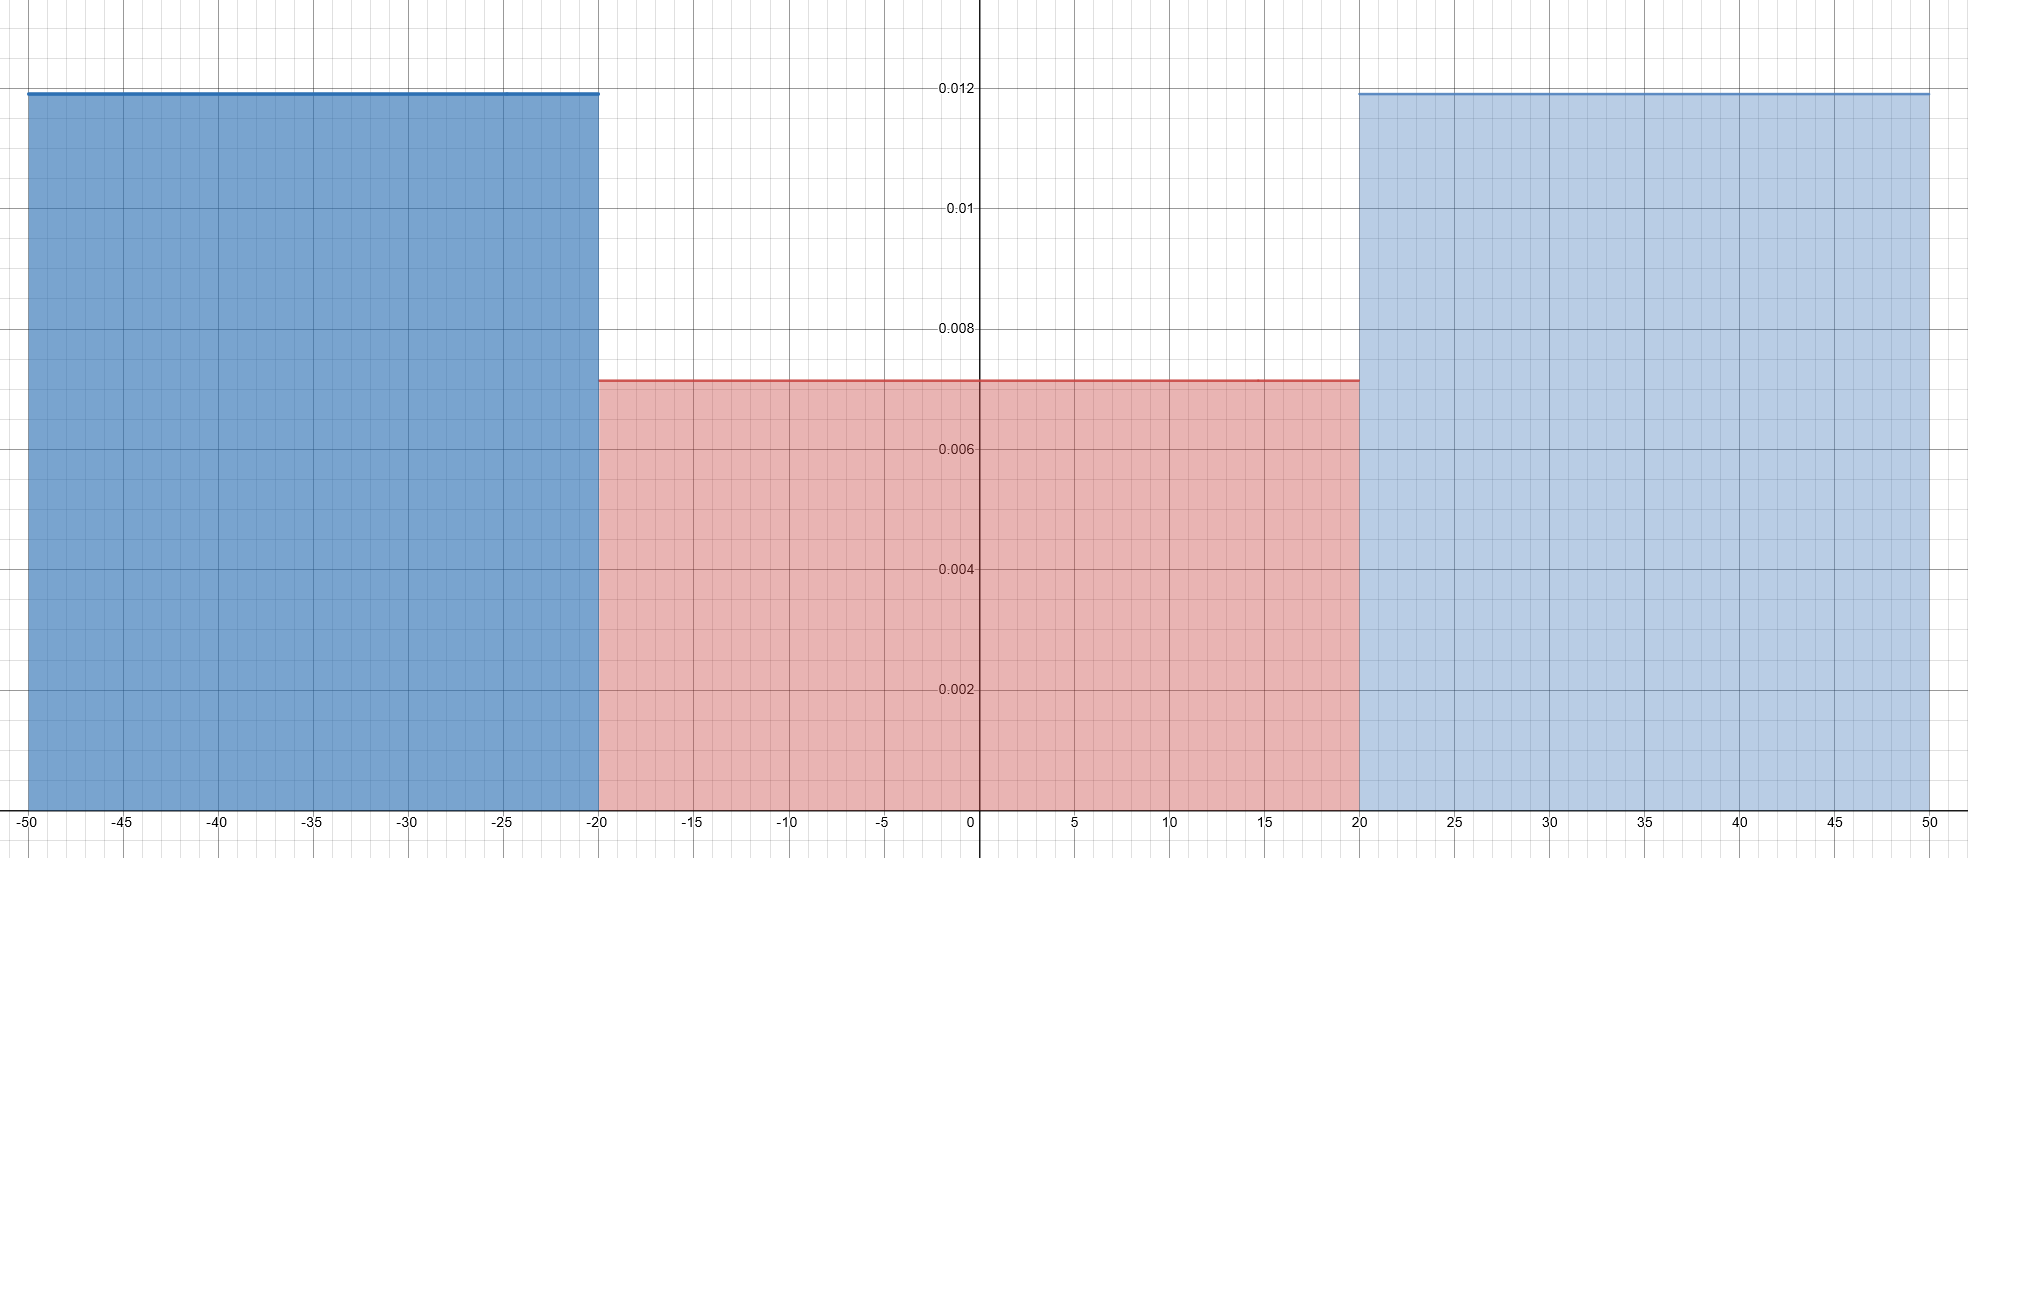
\includegraphics[scale=.3]{image.png}

\newpage 

\item What is the pdf of $\rx$ conditioned on $\ry$? Sketch it. 
\subitem To compute the conditional pdf we'll need to calculate the marginal first. Lets compute it firstly for y in $[-50,-20]$ which since it's symmetric will also work for y in $[20,50]$:
$$
    f_{x|y}(x|y) = \frac{f_{x,y}(x,y)}{f_y(y)} = 
    \begin{cases} 
    \frac{1}{100} & \text{when } -50 \leq x \leq 50 \\
    0 & \text{otherwise} 
    \end{cases}
$$
Now lets calculate it for y in $[-20,20]$:
$$
    f_{x|y}(x|y) = \frac{f_{x,y}(x,y)}{f_y(y)} = 
    \begin{cases} 
    \frac{1}{60} & \text{when } -50 \leq x \leq -20 \text{ or } 20 \leq x \leq 50 \\
    0 & \text{otherwise} 
    \end{cases}
$$

\begin{figure}[h!]
    \centering
    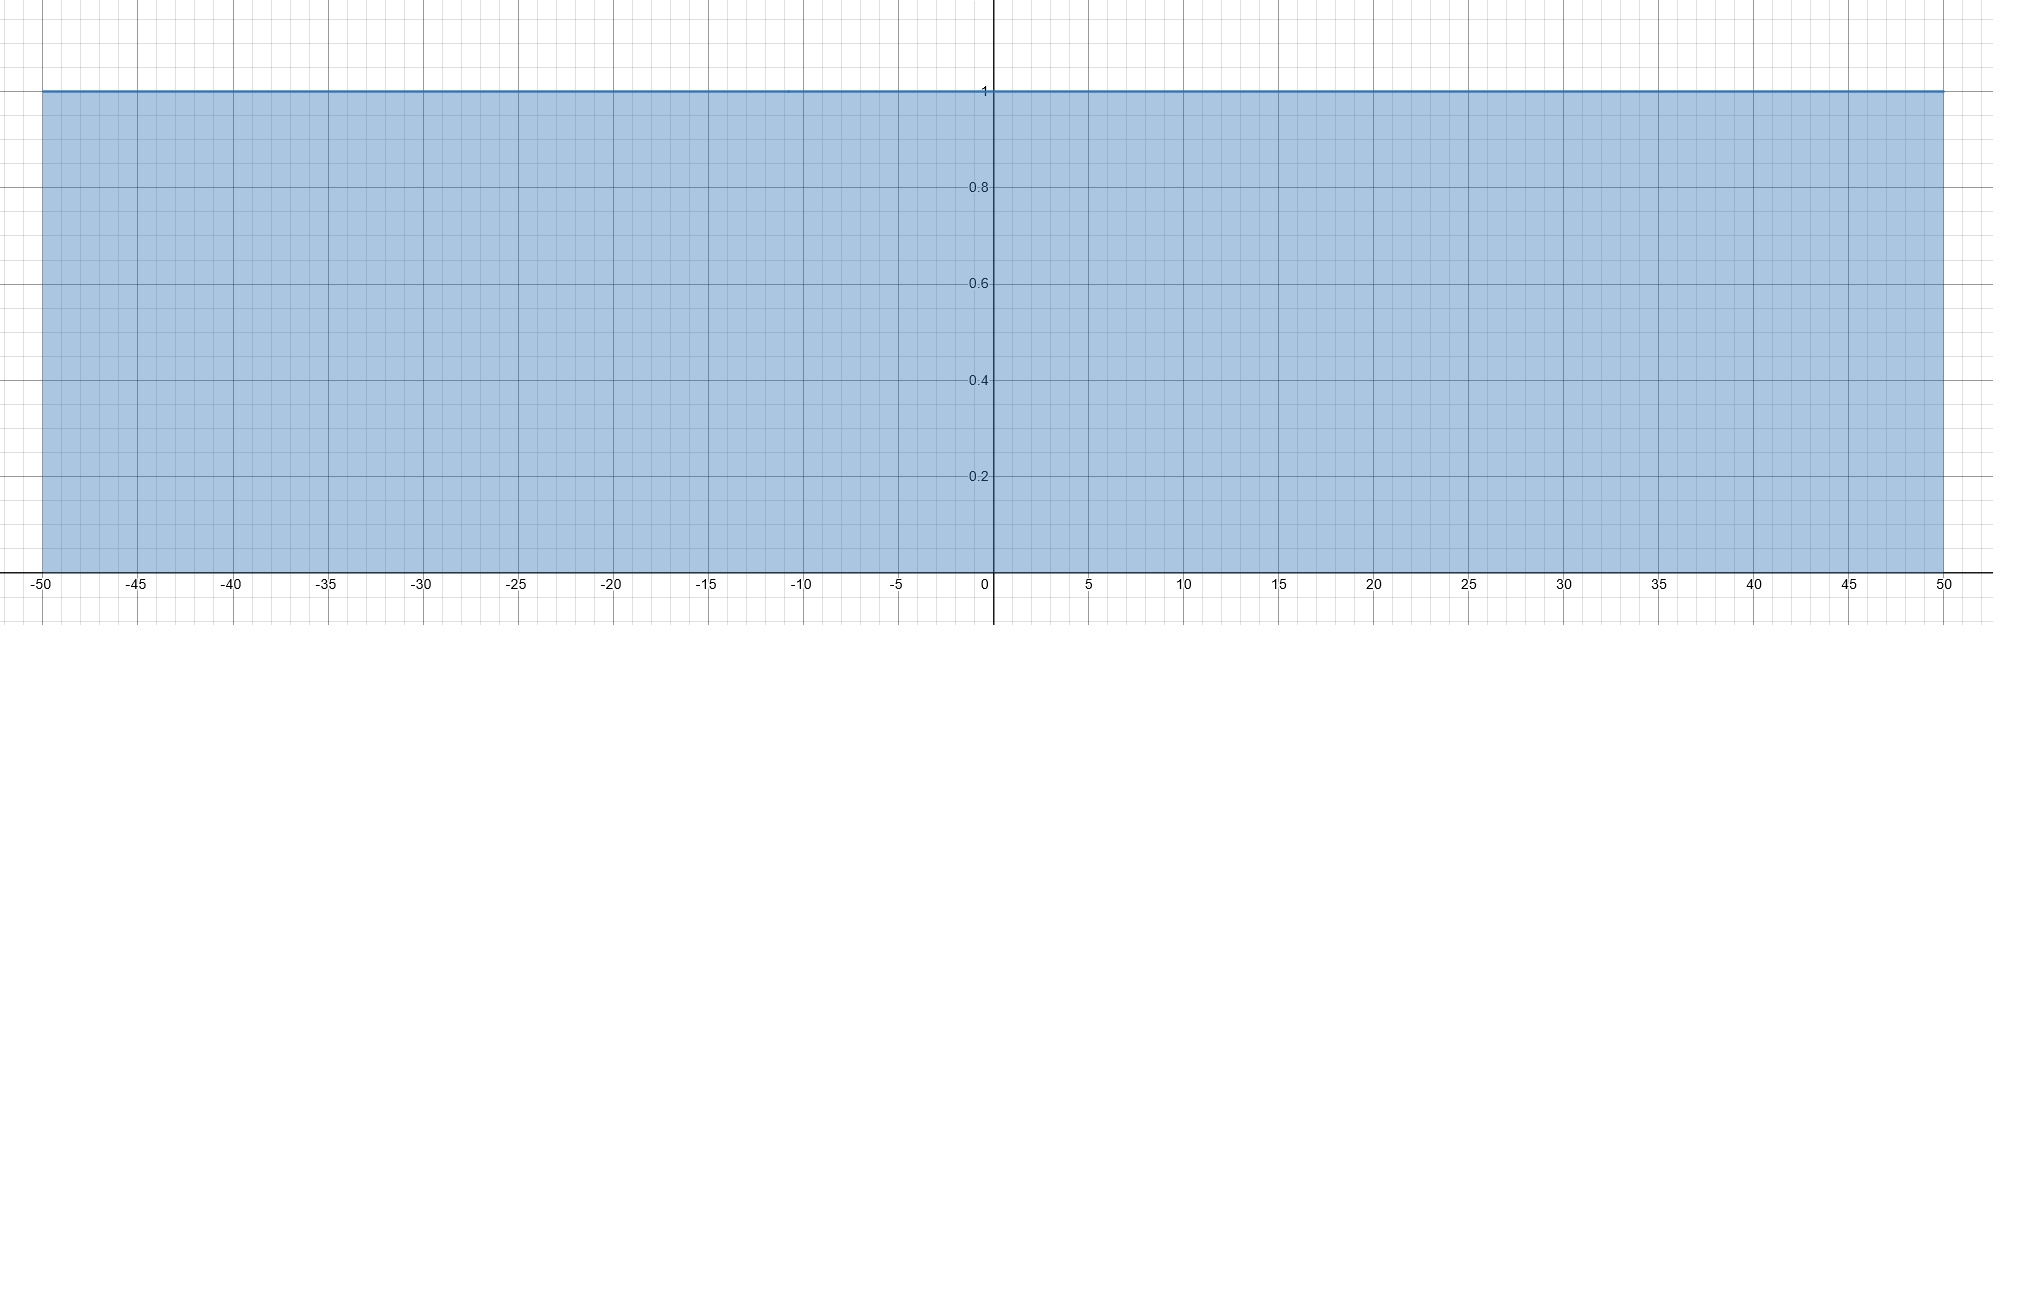
\includegraphics[scale=.2]{image2.png}
    \caption{PDF when y in $[-50,-20]$ or $[20,50]$:}
    \label{fig:my_label}
\end{figure}

\begin{figure}[h!]
    \centering
    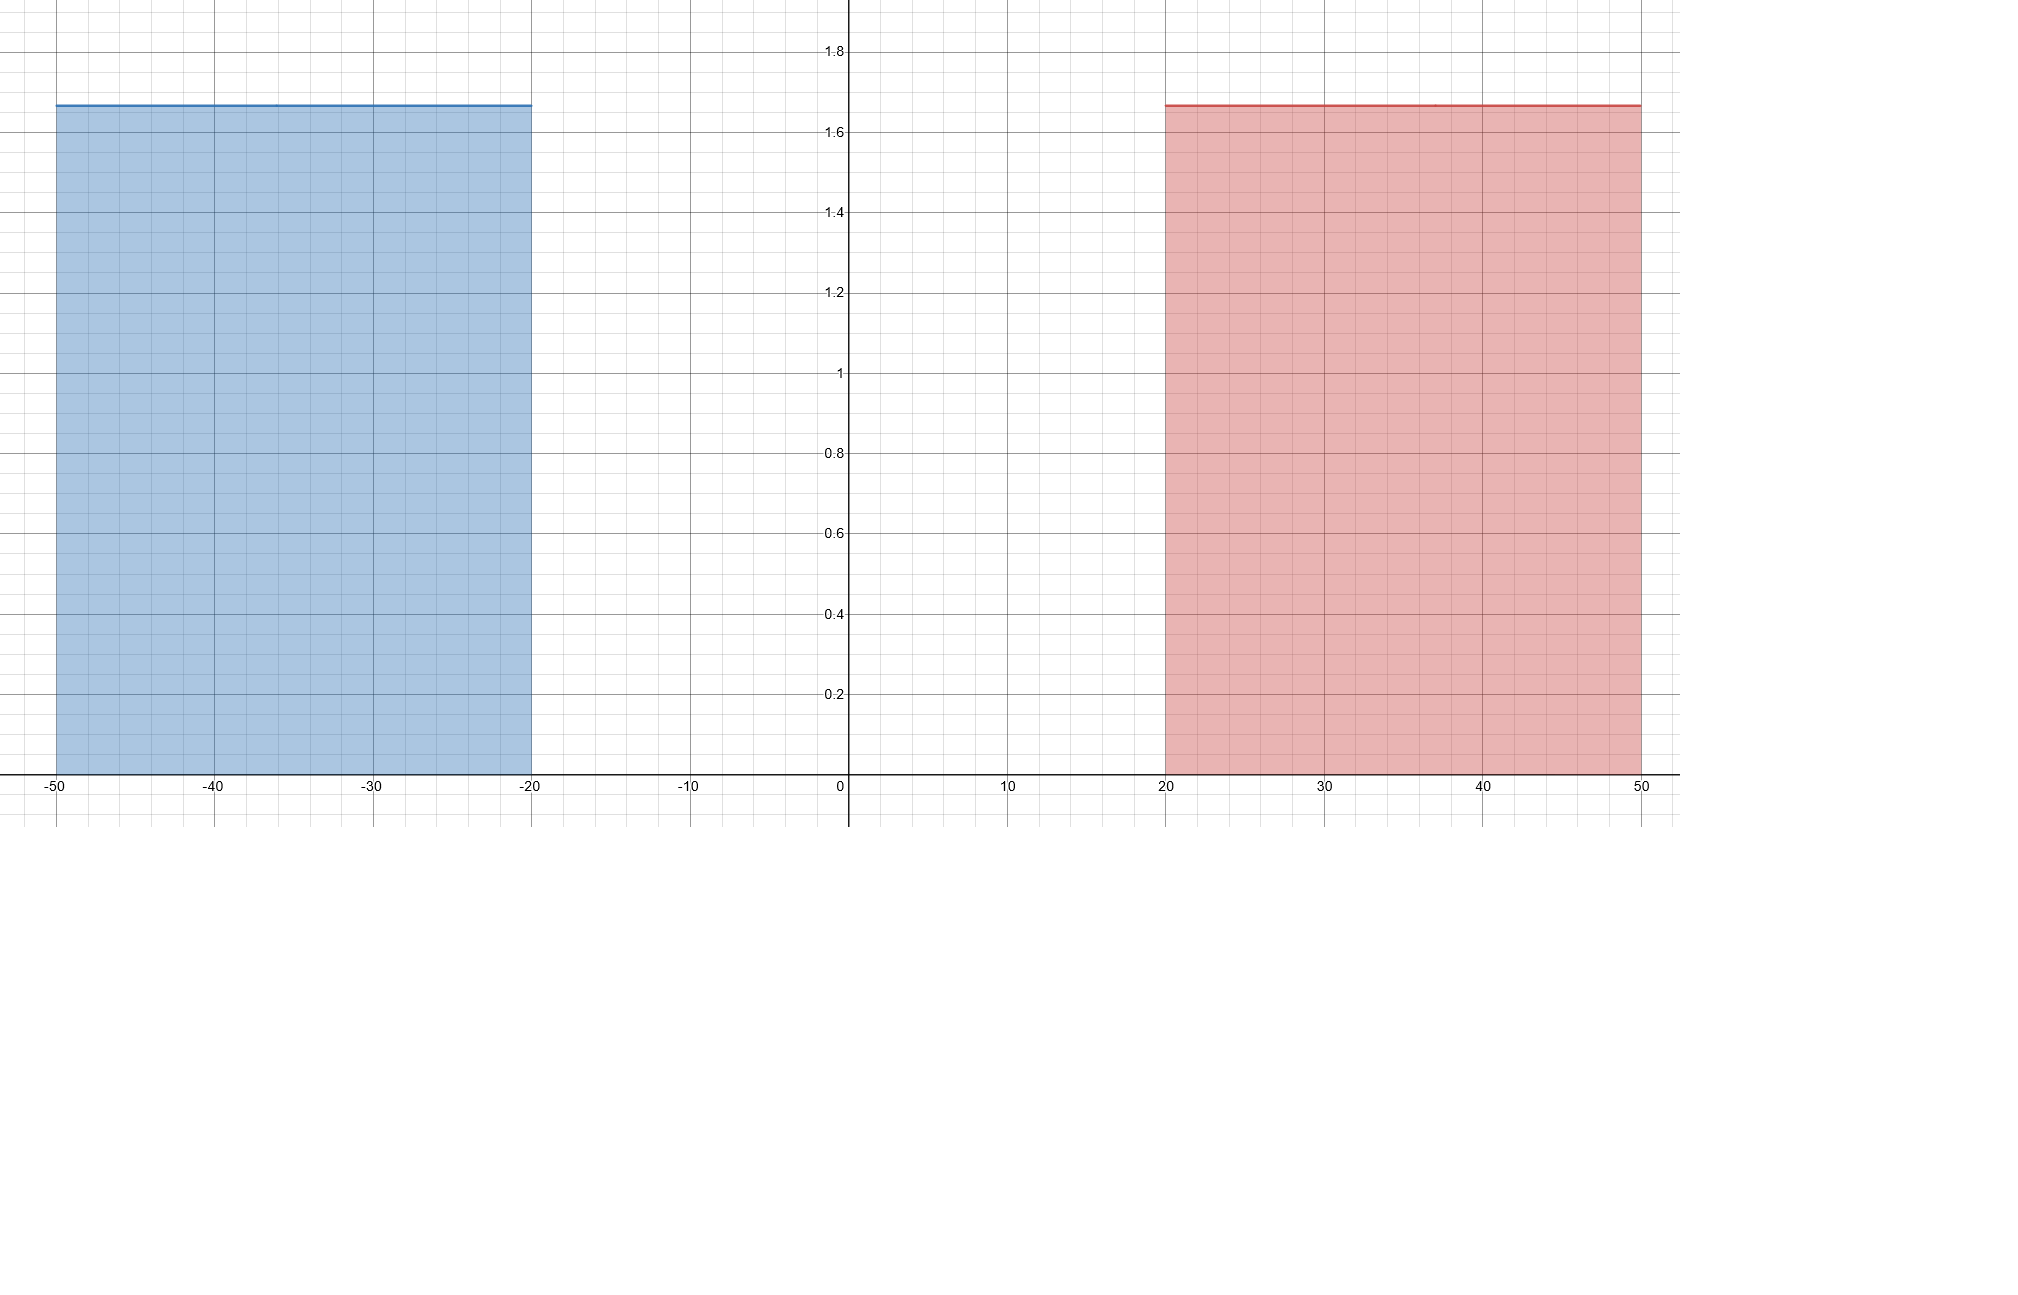
\includegraphics[scale=.2]{image3.png}
    \caption{PDF when y in $[-20,20]$:}
    \label{fig:my_label}
\end{figure}

\newpage

\item Are $\rx$ and $\ry$ independent? Justify your answer. 
\subitem We know that $\rx$ and $\ry$ are not independent as the distribution of x and y changes as you find out information about either variable.
$$
    f_{\rx,\ry}(0,0) \neq f_{\rx}(0) f_{\ry}(0)
$$
\item Are $\rx$ and $\ry$ uncorrelated? Justify your answer. 
\subitem $\rx$ and $\ry$ are indeed uncorrelated, which feels counter intuitive but once you analyze the mean and the variance of each random variable it comes clear. The mean of both $\rx$ and $\ry$ is 0, as they are centered about 0 and symmetric. Therefore, we only need to compute $E(xy)$ to calculate correlation via iterated expectation:
$$
    E(xy|y) = \int_{x=-50}^{x=50} \frac{xy}{100}dx = \frac{xy}{100}\int_{x=-50}^{x=50} xdx = 0
$$
This also works for the other bound: 
$$
    E(xy|y) = \frac{1}{60} (\int_{x=-50}^{x=-20} xdx + \int_{x=20}^{x=50} xdx)  = 0 
$$
Thus the two random variables are uncorrelated as their covariance is 0. 
% \item Given two independent samples from a uniform random variable equal to 0.1 and 0.3, generate a sample from $\rx$ and $\ry$. 
\end{enumerate}

\item (Random vector) 
A random vector $\rx$ with zero mean has a covariance matrix $\Sigma_{\rx}$ with the following eigendecomposition:
\begin{equation}
\Sigma_{\rx} = 
  \begin{pmatrix}
1 & 0 & 0 \\ 
0 & \frac{1}{\sqrt{2}} & \frac{1}{\sqrt{2}} \\
0 & \frac{1}{\sqrt{2}} & -\frac{1}{\sqrt{2}} 
\end{pmatrix}
\begin{pmatrix}
1 & 0 & 0 \\ 
0 & 0.5 & 0 \\ 
0 & 0 & 0
\end{pmatrix} 
\begin{pmatrix} 1 & 0 & 0 \\ 
0 & \frac{1}{\sqrt{2}} & \frac{1}{\sqrt{2}} \\ 
0 & \frac{1}{\sqrt{2}} & -\frac{1}{\sqrt{2}} 
\end{pmatrix}  
\end{equation}

\begin{enumerate}
\item What is the variance of each of the entries of the random vector $\rx[1]$, $\rx[2]$ and $\rx[3]$?

\subitem We can calculate the covariance matrix by doing the above matrix factorilization given in the problem statement. When we analyze the diagonal values of the resulting matrix, we'll have the variance of each random variable. When we do we find that the variance of $\rx[1]$, $\rx[2]$ and $\rx[3]$ is equal to $1,0.25,0.25$ respectively.
\begin{equation}
\Sigma_{\rx} = 
  \begin{pmatrix}
1 & 0 & 0 \\ 
0 & \frac{1}{\sqrt{2}} & \frac{1}{\sqrt{2}} \\
0 & \frac{1}{\sqrt{2}} & -\frac{1}{\sqrt{2}} 
\end{pmatrix}
\begin{pmatrix}
1 & 0 & 0 \\ 
0 & 0.5 & 0 \\ 
0 & 0 & 0
\end{pmatrix} 
\begin{pmatrix} 1 & 0 & 0 \\ 
0 & \frac{1}{\sqrt{2}} & \frac{1}{\sqrt{2}} \\ 
0 & \frac{1}{\sqrt{2}} & -\frac{1}{\sqrt{2}} 
\end{pmatrix}  =
\begin{pmatrix}
1 & 0 & 0 \\ 
0 & 0.25 & 0.25 \\ 
0 & 0.25 & 0.25
\end{pmatrix} 
\end{equation}


\item Is it possible to find a unit-norm vector $u$ such that the inner product between $\rx$ and $u$ (i.e. the amplitude of the projection of $\rx$ onto that direction) has variance greater than 1?
\subitem Since we are given the eigenvalues and eigenvectors from the covariance matrix eigen decomposition, we can see that the largest eigenvalue is 1. If we take a unit-norm vector and project it via inner product between $x$ and $u$ to achieve maximum variance, we see that the most we can amplify or scale the vector is $1$. Therefore, we cannot have a variance greater by $1$ as $1\times 1 = 1$.

\item Find three constants $a_1$, $a_2$ and $a_3$, such that at least one of them is nonzero and $P(a_1 \rx[1]+ a_2 \rx[2] + a_3 \rx[3] = 0) = 1$. Justify your answer mathematically, and interpret it geometrically.  
\subitem 
This problem is bascially asking "can we create the 0 vector for some (non-zero) linear combination of our random variables" which is the same as calculating a null space in linear algebra. Since random variables 2 and 3 are correlated 1:1 which I will show below, we can combine the two in a linear combination such that the result is alawys the 0 vector (this includes random variable 1 with scalar 0). Therefore the answer is: $a_1 = 0, a_2 = 1, a_3 = -1$
$$
    P( 0\times  \rx[1]+ 1 \times \rx[2] + -1 \times \rx[3] = 0) = 1
$$

We know this will work because $\rx[2]$ and $\rx[3]$ are correlated 1:1 as shown below:
$$
    Corr_{2,3} = \frac{cov(a,b)}{\sigma_a \sigma_b} = \frac{.25}{.5\times .5} = 1
$$
\end{enumerate}

\item (Financial data) In this exercise you will use the code in the findata folder.
  For the data loading code to work properly, make sure you
  have the pandas Python package installed on your system.

  Throughout, we will be using the data obtained by calling
 \verb|load_data()| in \verb|findata_tools.py|.  This will
  give you the names, and closing prices for a set of 18 stocks over a
  period of 433 days ordered chronologically.
  For a fixed stock (such as msft), let
  $P_1,\ldots,P_{433}$ denote its sequence of closing prices ordered in
  time.  For that stock, define the daily returns series $R_i:=P_{i+1}-P_i$ for
  $i=1,\ldots,432$.  Throughout we think of the daily stock returns as features,
  and each day (but the last) as a separate datapoint in $\R^{18}$.
  That is, we have $432$ datapoints each having $18$ features.
  \begin{enumerate}
  \item Looking at the first two principal directions of the
    centered data, give the two stocks with the largest
    coefficients (in absolute value) in each direction.  
    Give a hypothesis why these two stocks have the largest
    coefficients, and confirm your hypothesis using the data.  The file 
 \verb|findata_tools.py| has \verb|pretty_print()|
    functions that can help you output your results.
    You are not required to include the principal directions in
    your submission.
    \subitem
    In the first two principle components, Amazon and Google both have the highest weighted. This is because they each have large variance, but also have large share prices so they generate larger daily returns, thus skewing the weightings of the variance. 
  \item Standardize the centered data so that each stock (feature) has
    variance 1 and compute the first 2 principal directions.  This is
    equivalent to computing the principal directions of the
    correlation matrix (the previous part used the covariance
    matrix).  Using the information in the comments of
   \emph{generate\_findata.py} as a guide to the stocks, 
    give an English interpretation of the first 2 principal directions
    computed here. 
    You are not required to include the principal directions in
    your submission.
    \subitem
    After we center / standardize the data, and calculate the principle components, our first two PCs are much more interesting. The first principle component applies heavy weighting to the following stocks: SPY (S\&P 500 ETF) which indicates its variance is driven by the variance of the overall stock market, and its returns are generated by market movements.
    The second principle component applies heavy weighting to the following stock: USO, which is oil commodities. We can interpret the two principle components in the following way: when investors are bullish, the market rises, hence the first principle component. When investors are bearish, the stock market sinks, and oil which is seen as a hedge, and tends to spike when market conditions are subpar, rises.
  \item Assume the stock returns each day are drawn independently from a
    multivariate distribution $\rx$ where
    $\rx[i]$ corresponds to the $i$th stock.  Assume further that
    you hold a portfolio with $200$ shares of each of appl, amzn, msft, and
    goog, and $100$ shares of each of the remaining 14 stocks in the
    dataset.  Using the sample covariance matrix as an estimator for
    the true covariance of $\rx$, approximate the standard deviation of
    your 1 day portfolio returns $\ry$ (this is a measure of the risk of your
    portfolio).  Here $\ry$ is given by
    $$\ry := \sum_{i=1}^{18} \alpha[i] \rx[i],$$
    where $\alpha[i]$ is the number of shares you hold of stock $i$.  
    \subitem $$\ry := \sum_{i=1}^{18} \alpha[i] \rx[i] = 6962$$
    
  \item Assume further that $\rx$ from the previous part has a
    multivariate Gaussian distribution.  Compute the probability
    of losing $1000$ or more dollars in a single day.  That is,
    compute
    $$\Pr(\ry \leq -1000).$$
    \subitem 
    The expected daily return from our portfolio is $879.78$. Since we have the variance and mean of our porfolio, we can now calculate the probability of losing more than $1000$ a day using a normal distribution. The probability is approximately $39.36\%$
  \end{enumerate}
  Note: The assumptions made in the previous parts are often
  invalid and can lead to inaccurate risk calculations in real
  financial situations. 

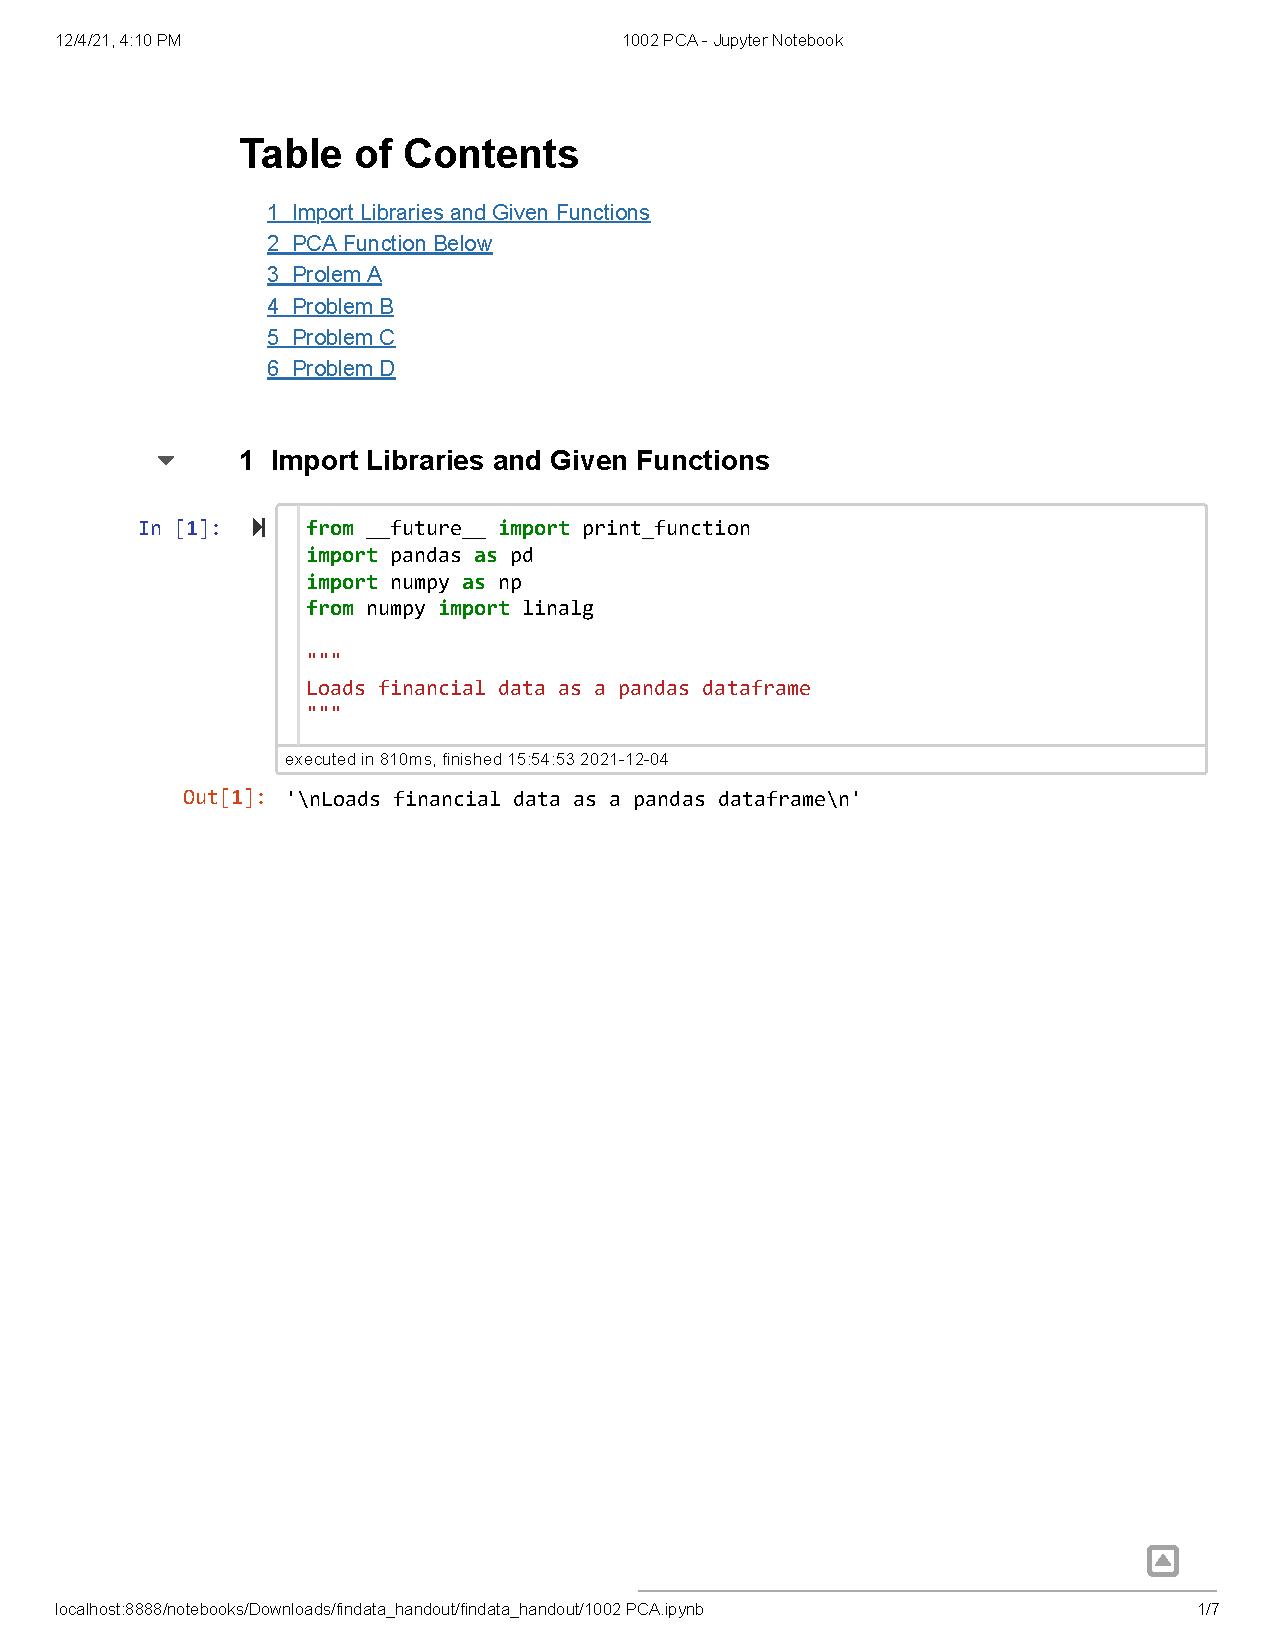
\includepdf[pages=-]{pca.pdf}
\end{enumerate}
\end{document}
